\documentclass[]{report}

\usepackage[square, numbers]{natbib}
\usepackage{hyperref}
\usepackage{url}
\usepackage{graphicx}
\usepackage{caption}
\usepackage{subcaption}
\usepackage[english]{babel}
\usepackage{enumitem}
\usepackage{array}
\usepackage{lscape}
\usepackage{gensymb}


% Title Page
\title{Software Design Study\\Final Report}
\author{Jack Browne, 1236782\\Thomas Clarke, 1162927\\Keiran Crook, xxxxxxx}


\begin{document}
\maketitle

\tableofcontents

\chapter{Introduction}
\section{Problem Definition}
%Rest of page on why we chose this problem space
%Key statistics
We began this project by exploring the 'Safety in Cycling' problem space. Our motivation for exploring this space came from looking at the reasons why people do not cycle. Even though cycling is a fairly easy form of exercise and an environmentally friendly method of transport just 2\% of trips are made by bicycle\cite{travelsurvey}. We feel that this figure is way too low and should probably be closer to the 10\% mark to bring the UK in line with the rest of Europe.

Investigating this, we looked at some of the reasons why people choose not to cycle in the UK and the general trend was that people thought cycling was not safe enough. For example, a question in a Transport for Greater Manchester survey asked ``Which of the following do you feel are the barriers to cycling?" and 74\% of respondents said `Road Safety'\cite{TfGM}. In a similar survey by the Department for Transport 61\% of people either definitely agreed or tended to agree with the statement ``It is too dangerous for me to cycle on the roads"\cite{dft}.

In fact, interestingly, when comparing fatalities there is actually more risk being a pedestrian than a cyclist. This may be evidence that the problem is more about `subjective safety' rather than absolute risk. 

Safety is quite a wide term so we had to speak to different stakeholders and analyse some statistics to really see the reasons \textit{why} cycling is not safe (or at least not considered to be safe). From this research we were able to narrow the problem down to the following:

\begin{itemize}
  \item Reducing the number of accidents on UK roads, with a particular focus on commuting hours. The majority of accidents occur during these hours; likely because of the increased traffic causing car drivers to become frustrated and/or make mistakes. 
  \item Improving the perception of cycling to be a safe mode of transport. This is to address the `subjective safety' issue. A successful solution to this should not only make the cycling safer but the safety improvement should be clear and obvious to the cyclist themselves. We believe that this is reason why, although accident numbers are falling, current safety products have not seen the number of cyclists dramatically increase.
\end{itemize}
%Maybe this section can go
\section{Purpose}
This report is written for the benefit of any software or hardware engineers who are tasked with implementing this product. For this reason, in parts, the report may assume some basic technical knowledge of these fields. For example, understanding of the UML diagrams used in section ?.

The report should describe, in detail, our solution to the problem above. The detail should be enough so as that a small team of people would be able to implement the solution in its entirety with relative ease. The report should address all of they key areas of the solution and be void of any ambiguities so that it alone can clarify any queries about the product.

As well as this, the report will show the progression of our ideas and the steps taken to reach our final design. Throughout the design of this product we reached points where we had to make a justified decision from a range of possibilities. We always tried to make a rational decision based on the information available coupled with our in-depth knowledge of the problem space. Each of these key decisions will be described in detail for the benefit of the reader.

\section{Overview}
Firstly this report will give a rough outline of the solution that we came up with and why we decided to go with that particular solution as well as some of the features we considered but ultimately decided not to include. This will help to give some context to sections of the report that follow.

Before discussing the details of the design we will outline some of the things we had to take into consideration before designing our solution. Including the overall design goals that we were following throughout.

In the later sections of the report we will describe in detail the overall architecture of the product and how the main components of the system will work. Many of these components are either amalgamations of the best features of the similar products on the market or involved a choice between different ideas. For all of these cases we will describe in some detail all of the different options that we had and then our reasons for choosing a particular one over another.

Finally we will present our critical analysis of the prototypes that we created and show how using this analysis we iterated on the prototypes to reach to our final design.

\section{Definitions, Acronyms and Abbreviations}
\begin{description}
\item[RTA] Road Traffic Accident
\item[UCI] Union Cycliste Internationale
\end{description}
\section{References}
The design decisions that we made are based on our earlier research and we will continually refer to this research throughout the report, all of which is documented in the Research Report found in the appendix. 

All other papers, articles, etc. that were used to formulate our ideas are referenced in the Bibliography.

\chapter{System Overview}
% 2 or 3 pages on what the finished syetem does
% Intended users
% Key features and why
% Rejected features and why
After fully analysing the problem space we came up with an idea for a product that we felt solved the key issues around bike safety. As with most modern products, ours is heavily influenced by new technologies; particularly automation systems in cars culminating in the recent development of self-driving cars. % Reference Google project

The core of our product is a collision avoidance system revolving around automated braking. In general the bike should be capable of analysing other road users, predicting the likelihood of a collision occurring and then applying the necessary amount of braking. The technology for performing this task in cars is fairly well developed and becoming more and more widely deployed, for example the Subaru EyeSight\cite{eyesight} and a similar system developed by Volvo\cite{volvo}. However there is no such system for road bikes. This is probably due to the computing power needed and a bikes natural instability. We believe that these problems can be overcome with some careful design.

We decided this should be a fully integrated bicycle rather than a set of accessories for somebodies existing bike. The primary reason for this is to help overcome the instability issue. An additional reason is that it allows us to incorporate a wider range of sensors than would be feasibly possible in an accessory kit. This does have the disadvantage that some people may have already spent a large sum of money on their current bike and may not want to part with it.


To interface this system there will be a smartphone application, enabling users to customise their settings and have them automatically download whenever they get on the bike. As well as this, the smartphone app will provide some performance information to the user as they are cycling such as current speed and the current battery level of the bike.

\section{Rejected features}
During our research we discussed a multitude of different solutions (or parts of solutions); some of which were very similar to our final design and some which are markedly different. Many of these solutions were rejected reasonably quickly while others were still being discussed during later iterations of the design. However all of the ideas below were eventually rejected because they were either unsuitable or unnecessary.

\paragraph{Safety based route planner} An idea that was considered for a long time was a route planning application. This was intended to work alongside the collision avoidance system as part of an wider ecosystem of safety technologies. Core to this would be crowdsourcing information from all other road users; traffic speeds, accidents, road conditions, etc.. All of this information could then be combined and analysed in order to provide the cyclist with the safest route. We deemed the safest route to be: 
\begin{enumerate}
\item One with less traffic, as discovered from research [enter research], there was a positive correlation between increased traffic and increased cyclist accidents. 
\item One which avoided areas with a certain risk level, both short and long term. A known accident blackspot might be a long term risk. If an accident has just occurred then the surrounding area might be a short term risk.
\item One which took environment factors into consideration, that were deemed a risk to cyclist. For example poor road conditions, poor weather conditions, high pedestrian activity, etc.
\end{enumerate}
 
This was an idea that we invested a lot of time into and one that we still believe under the right conditions could be very successful. However, for our project we decided to drop this feature because:
\begin{itemize}
\item It was too dependent on other users to enable it to offer what we wanted. Car drivers needed to use the application and we did not think enough drivers would be willing to share all of the necessary information for something that provides them with little benefit.
\item It would require too many sensors and additional components for it to be a viable option. This could be overcome by having it as part of an integrated bicycle however in this case we would likely not have the required number of users for it to be successful.
\end{itemize}


\paragraph{Wearable tech}As a group we very quickly latched onto the idea of incorporating wearable technology into our final solution - particularly inspired by recently evolving wearable eyewear technology such as Google Glass. We felt that one of the problems we would eventually have is that a bike has no significant interface/dashboard and wearable eyewear is a very natural solution to this problem. The other interface solutions that we came across were: 
\begin{itemize}
  \item a smartphone mounted on the handlebars
  \item a small on-board-computer
  \item more recently, smartwatches
\end{itemize}
However all of these have the same fundamental problem; they require the cyclist to divert their attention away from the road. Lack of attention, from either party, is one of main causes of RTAs involving bicycles. %statistic!

In spite of all this we decided to forget this idea following a user-review. Several of the people failed to grasp the concept. Firstly not many people have access to any wearable eyewear technology at present so designing an integrated bike along with an app for an existing eyewear platform is not really feasible. The other alternative would be to design a piece of eyewear technology to use for along with any existing bike however the number sensors that would need to be installed and calibrated means that for most people this simply isn't practical.

\paragraph{Self inflating tyres} An idea that was briefly considered was self inflating tyres. Inspired by similar technology in cars where the tyres will inflate or deflate depending on the current speed or road conditions. Following our research we found that a vaguely similar technology for bikes is currently in development by a San Francisco company PumpTires\cite{pumptyres}. This technology looked promising and even made it into our first prototype.

However, a handful of users asked some interesting questions about this feature which after some consideration prompted us to drop it. When really considering what this feature adds to the overall system we realised that it doesn't really contribute much but drives up the cost vastly. The core of our system is the collision avoidance; self inflating tyres don't really help us to achieve that and in reality this was just a leftover feature from earlier discussion.

As well as this we realised that we had not properly thought through how to actually implement this. PumpTires have patented much of their technology and we don't really have the technical expertise required to invent a new solution. It is possible that we would be able to use PumpTires system directly, however it would be just as easy for people to do this themselves if this is a particularly important issue to them.

\chapter{Design Considerations}
\section{Assumptions}
% 2 pages on the above
% Assumptions about users (age, race, gender, disability)
% Assumptions about environment (road, many other users, etc.)
% Assumptions about interface (All users will have a phone)
% Constraints (Cost, weight/size)
When designing this system we have had to make a few assumptions about certain characteristics of the end users, this is because it would be almost impossible to design a system of this nature that is both effective and easy for everybody to use. 

Firstly we have assumed that the end user will be fully able-bodied. We feel that this is a necessary assumption despite the fact that one in twenty cycling commuters are disabled \citep{census-dis}. Cycling is a very physical activity and generally those with severe physical disabilities are better off with a bike that is specifically designed to cater for their particular disability. It is very much possible that our final design will be usable for the less severely disabled, however we will not be creating our design with any of these disabilities in mind. 

Secondly we will be assuming that end users have some familiarity of bikes, particularly road bikes. By this we mean that we will not be designing an educational tool that teaches people how to ride a bike nor an assistance tool that aids those who cannot already ride a bike. This is a reasonable assumption because it would be against recommended practice for a non-cyclist to start out by cycling on main roads anyway. %Who's recommended practice? Sources?
In fitting with both of the above assumptions, we will also be assuming that the bike is to be used only by fully grown adults.

The majority of our research has been based around cycling in the UK for two reasons:
\begin{enumerate}
  \item We are based in the UK, giving us much easier access to end-users (UK cyclists)
  \item Although we didn't look too deeply, our research suggested that many European countries actually have a fairly good cycling population
\end{enumerate} 
Because of this our product will be designed to be used on UK roads. We will make no further assumptions about the environment it is used in. The final product should function on busy city roads, country lanes or quiet residential roads with the same effectiveness. We will not be designing the product to work with any other system of roads (European, American, etc.) but it is highly likely that with some minor adaptations this product could function on any road system.

The final assumption we had to make came about as the result of a discussion following our initial prototype. We assumed that all of our users would have a smartphone. The reasons for making this assumption are discussed in detail in section \ref{sec:phones}. We feel that this was a reasonable assumption because there are an estimated 37.8 million smartphone users in the UK\cite{smartphones}. This is a huge percentage of the adult population that we are aiming at.

\section{Constraints}
There are some overall restrictions that the product naturally has in order for it to be feasible or usable. The main two that we considered were:
\begin{itemize}
  \item \textbf{Cost} because in order for a solution to be considered suitable it must be available to the general population of commuting cyclists. A solution that does everything that we set out to achieve but could never be purchased by even the richest of cyclists could not be considered suitable.
  \item \textbf{Weight} because this has a significant impact on whether the bike is actually ridable. We want to design a solution for which it is, not only possible but, comfortable to ride on the majority of commuting roads. Some of which will involve steep inclines.  
\end{itemize}
\subsection{Cost}
We are attempting to create a solution for the average commuting cyclist to use on the road. This means it is important that the average commuting person is able to afford the product. To do this we must be able to find the right components and produce the bike for a reasonable cost. To decide what constitutes 'reasonable' we analysed how much cyclists currently spend on their bikes and asked cyclists how much they would be willing to spend on a bike of this style/quality.
\begin{figure}
\centering
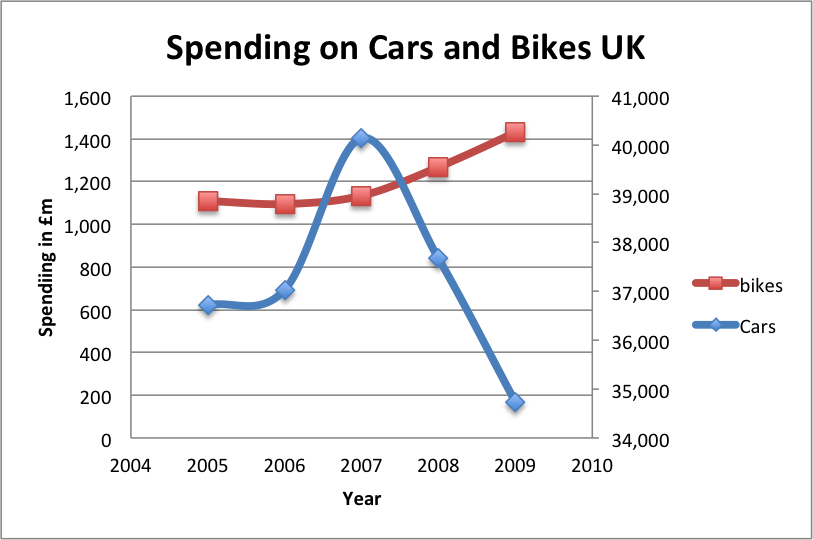
\includegraphics[scale=0.9]{figures/cars-bikes-spending}
\caption{Graph showing the retail sales of cars and bikes \cite{uk-stats}}
\label{fig:cars_bikes_spending}
\end{figure}
\paragraph{Current spending}
Overall spending on bikes is slowly increasing at the same time as spending on cars rapidly decreasing as shown by figure \ref{fig:cars_bikes_spending}.Possibly indicating a   However, last year in the UK, the average amount a person spends on buying a bike was only £233. However, this statistic is likely skewed by the large amount of cheap bikes sold to casual cyclists; these are not the people we are aiming this product towards\cite{spending-more}. There are no readily available statistics that differentiate between the spending on road bikes and otherwise but we were able to get a fairly good idea using statistics from the Cycle to Work scheme - which allows people to buy commuting bikes and equipment tax free. This saw commuters spending an average of over £1,100\cite{spending-more}. This is more in line with the price our bike would retail for and the cyclists we are aiming at. As well as this, our earlier research found that commuters spend a further £195 on accessories alone, many of which may be incorporated directly into our design.

\begin{figure}
\centering
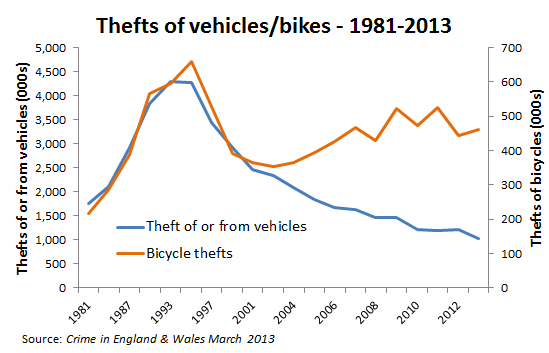
\includegraphics[scale=0.8]{figures/cycle-theft}
\caption{Graph showing the thefts of vehicles and bikes \cite{ctc-stats}}
\label{fig:theft_graph}
\end{figure}
\paragraph{Concerns}
As can be expected; cyclists are always concerned about the theft of their bike. Strangely, thefts of or from cars and other vehicles has been steadily decreasing since the late 90s. While in that time thefts of bicycles has generally increased (Fig. \ref{fig:theft_graph}). This is a worrying trend and may be a contributing factor to people opting for cheaper bikes.

However, we can reasonably assume that consumers who spend more on their products will be  willing to spend a little extra on security or insurance. This might go some way to counteracting the concern about theft. Another way to alleviate these concerns might be to incorporate anti-theft devices into the product itself, similarly to ‘Find my iPhone’ and similar products.
\paragraph{Conclusion}
From the research we decided that an appropriate cost for producing this bike is \pounds1000. Even though this is significantly more than the average spend for a bike we feel that it is justified for a product of this quality since it is in the region that cycling commuters currently spend (particularly once accessories are taken into account). Also, this still comes at considerably less cost than many of the commuting alternatives (diriving, public transport,etc).

\subsection{Weight}
There are not many statistics out there regarding the weight of consumer bicycles so most of this research came from talking to cyclists and cycle shops.
\paragraph{Current products}
UCI impose a minimum weight of 15 lbs, for this reason many cyclists consider anything around this weight or lighter to be a \textit{light} bike. However, the retailers that we spoke to were generally of the opinion that bikes at this end of the scale were only really appropriate for competitive racing environments. They thought that 23 lbs was a good weight for a road bike or 30 lbs for a more general purpose mountain bike. These weights give a good trade off between speed and ease of ride.

\paragraph{Electric bikes}
Working with the 23 lb ballpark figure, as suggested by the cycling retailers that we spoke to, we noticed a problem. Given that this product heavily relies on a computer performing some calculations and some sensors feeding information into the computer we clearly will require some sort of battery. Looking at the current bike batteries on the market this would not be easy to fit into our 23 lb restriction. In the Specialized Turbo S, for example, the battery alone weighs 8 lbs\cite{turbo-s}. This would take up over $ \frac{1}{3} $ of our weight limit. This doesn't leave much room for a frame, wheels and pedals; let alone sensors and a computer. When all of this is factored in, we are realistically looking at a minimum of 45/50 lbs. This is likely to be almost to twice the weight that many cyclists are used to and as a result may be very difficult to ride. The obvious solution to this problem is to heavily assist the cyclist with a motor powering the wheels. This is the primary use case for current electric bikes so the technology already exists and shouldn't be too difficult to implement

\paragraph{Conclusion}
Cyclists have a reputation for being obsessed with weight - trying to shave off pounds at every opportunity. However our research showed that most commuters probably wouldn't be overly concerned about a slight increase in weight if it meant an equally good (or better) performance and a more comfortable ride. This makes sense because, in reality, the cyclists themselves are usually by far the biggest contributor to the weight of the bike. Also, as a result of this research, it is likely that our final product will need contain some form of motor or other electronic assistance which will help to carry some of the weight. This puts our product more in line with electric bikes on the market, rather than regular road bikes. This gives some additional flexibility regarding the weight of the bike.

In conclusion we have decided that we will design the bike with a 60 lb restriction. This should allow us to include all of the hardware components that will be necessary for our solution, with the bike still being comfortable to ride. 

\section{Design Goals and Guidelines}
% 1 page on U(X/C)D and why this is suitable for our product
% Double diamond model (Design council)
\subsection{User Centred Design}
Our overall design goal was to come up with a product that was tailored to fit the needs of the end-user. In this case the end-users are cyclists (or potential cyclists). This was especially important for us because the whole idea was to design a product to make cyclists feel safe on the roads. In the User Centred Design process the end-user is involved at every single stage; we continually used the user opinions to formulate or improve our design.

A further consideration was the other stakeholders (a map of which can be found in appendix \ref{ch:stakeholders}). We had to consider these stakeholders as much as possible, for example car drivers might be able to offer some insight that cyclists cannot. It is not possible to get in touch with all of these stakeholders; we could not find anyone that openly admitted to being a bike thief for example.

Some of the User Centred Design methods that we used were:
\begin{description}
  \item[Questionnaires] This was our primary method for getting in touch with users. This was suitable for us because they are relatively cheap and easy to set up. Also cyclists are fairly easy to access which meant we had a large enough sample size to make the information from the questionnaires viable. Questionnaires are particularly good at getting statistical data. This was used predominantly in the requirements gathering stage however some smaller questionnaires were used to allow our user testers to give their feedback on our prototypes.
  \item[Interviews] We carried out a couple of informal interviews with a cycling retailer (Urban Cycles on the university campus). This was a suitable way for us to get in touch with retailers because the number of retailers we were able to talk to was fairly low. 
  Interviews gave us a qualitative opinion on a range of topics. This was good for us because we used these interviews to find out the latest trends and to get expert opinions. Interviews were predominantly used in the requirements gathering and early stages of the design phase.
  \item[Usability testing] We did some usability testing with end users to evaluate our prototypes. We asked people to perform some tasks using our prototype and recorded the time taken. This gave us a statistical measure of how efficient our design was. 
  
  We also watched them as they carried out the task to get a qualitative understanding of the particularly complex areas of the design. This was an evaluation technique.
\end{description}

\subsection{Double Diamond Model}
During this project we followed the Double Diamond design process as put forward by the Design Council\cite{doublediamond}. 

This process has four key stages:
\begin{description}
\item[Discover] In this stage we explored all elements of the problem space; gathering as much information as possible from a whole variety of sources. Statistics were used to give us the raw quantitative data that would be used to back up our views about the problem space, while questionnaires were used to get a more qualitative view. Also questionnaires gave us the opportunity to get opinions directly from potential users (or other stakeholders) of the system; helping the to achieve our goal of creating a user centred design.
\item[Define] Once we had gathered all of our information we then had to interpret it to accurately identify the contributing factors to cycling accidents, allowing us to focus our efforts in the right way. At this stage we also came up with a starting point for final product.
\item[Develop] It was during the development stage that we really investigated all of the different ways of achieving what we had envisaged. Here we had to consider what would be practical, how different components would interact and, most importantly, what actually works.
\item[Deliver] This stage was a series of prototype-feedback loops. We would come up with a prototype, scrutinise it for potential design flaws, adapt the design and repeat. This process continued up until the point where we had our final design.
\end{description}
\begin{figure}[h]

\centering
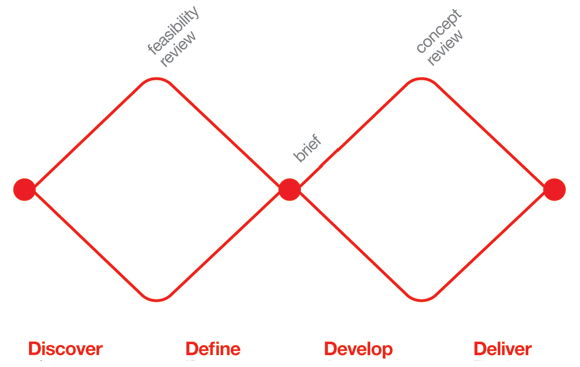
\includegraphics[scale=0.4]{figures/diamond}
\caption{A visual representation of the double diamond model}
\label{fig:diamond}

\end{figure}
\subsection{Agile approach}
We came up with a initial set of requirements during the define stage of the double diamond model - once we had our rough outline of how our solution would work. However these were very open to change. In keeping with our overall goal of creating a user centred design, we allowed the user feedback and prototype analysis to govern how the requirements of the product adapted and changed. 

In an agile approach such as this one the design is developed in small increments - starting from the 'minimum viable product' all the way up to the final design. An example of this is how we adapted our prototypes in chapter \ref{ch: prototype}. Without using an agile approach we would not have been able to go back and make these drastic changes to our design because they would most likely conflict with the initial requirements. The agile approach works very nicely within the User Centred Design guidelines.

\chapter{Specification}
In keeping with the agile approach that we took to the design the functional requirements are fairly high level and lacking in detail. This detail was realised in the use cases, shown in section \ref{sec:use-cases}.
\section{Functional Requirements}
\label{sec:func_req}
\begin{enumerate}[label=\ref*{sec:func_req}.\arabic*.,leftmargin=*]
\item The system should 
\begin{enumerate}[label*=\arabic*.]
\item The user should be able to customise the system behaviour easily
\end{enumerate}
\end{enumerate}
\section{Non-functional Requirements}
\subsection{Usability}
\label{usability}
\begin{enumerate}[label=\ref*{usability}.\arabic*.,leftmargin=*]
\item The system should be easy to use
\begin{enumerate}[label*=\arabic*.]
\item The user should be able to customise the system behaviour easily
\end{enumerate}
\end{enumerate}
\subsection{Efficiency}
\label{efficiency}
\begin{enumerate}[label=\ref*{efficiency}.\arabic*.,leftmargin=*]
\item The system should
\end{enumerate}
\subsection{Dependability}
\label{dependability}
\begin{enumerate}[label=\ref*{dependability}.\arabic*.,leftmargin=*]
\item The system should be available at all times
\begin{enumerate}[label*=\arabic*.]
\item The core of the system be usable without an internet connection
\end{enumerate}
\end{enumerate}
\subsection{Security}
\label{security}
\begin{enumerate}[label=\ref*{security}.\arabic*.,leftmargin=*]
\item The system should hold all customer information securely
\item The system should be secure from theft
\item The system should be secure from hackers
\end{enumerate}
\subsection{Environmental}
\label{environmental}
\begin{enumerate}[label=\ref*{environmental}.\arabic*.,leftmargin=*]
\item The system should be environmentally friendly
\end{enumerate}
\subsection{Operational}
\label{operational}
\begin{enumerate}[label=\ref*{operational}.\arabic*.,leftmargin=*]
\item The system should be suitable for people aged 16 and over
\end{enumerate}
\subsection{Development}
\label{development}
\begin{enumerate}[label=\ref*{development}.\arabic*.,leftmargin=*]
\item The system should be well documented
\begin{enumerate}[label*=\arabic*.]
\item All code should be properly commented
\item The
\end{enumerate}
\end{enumerate}
\subsection{Regulatory}
\label{regulatory}
\begin{enumerate}[label=\ref*{regulatory}.\arabic*.,leftmargin=*]
\item The system should conform to the Pedal Bicycles Safety Regulations (PBSR)
\item The system should comply with Statutory Instrument No. 1168 (1983)
\end{enumerate}
\subsection{Ethical}
\label{ethical}
\begin{enumerate}[label=\ref*{ethical}.\arabic*.,leftmargin=*]
\item The system should 
\end{enumerate}
\subsection{Legislative}
\label{legislative}
\begin{enumerate}[label=\ref*{legislative}.\arabic*.,leftmargin=*]
\item The system should comply with the Data Protection Act 1998
\end{enumerate}

\section{Use cases}
\label{sec:use-cases}

\chapter{Design Decisions}

\section{Communication}

\subsection{Wireless}

\begin{landscape}

\begin{table}[h]
\resizebox{1\textwidth}{!}{\begin{minipage}{\textwidth}

    \begin{tabular}{ | m{2.5cm} | m{2.5cm} | m{2.5cm} | m{2.5cm} | m{2.5cm} | m{2.5cm} | m{2.5cm} | m{2.5cm} |}
    \hline
    \textbf{Wireless comms} & \textbf{Max Data Rate} & \textbf{Security Protocol} & \textbf{Encryptionl} & \textbf{Connection Latency} & \textbf{Avg Power Consumption} & \textbf{Range} & \textbf{Backwards Compatible}\\ \hline
   
   Bluetooth v2.0 + EDR & 2.1 Mbit/s & & 128 bit stream cipher & & Class 1 radio: 100mW &   \\ \hline
   Bluetooth v2.1 + EDR & 3 Mbit/s & & 128 bit stream cipher & & Class 1 radio: 100mW & \\ \hline
   Bluetooth v3.0 HS & 24 Mbit/s & & 128 bit stream cipher & & & & \\ \hline

   
    \end{tabular}


\caption[Table caption text]{Wireless communication methods comparison} 
\label{table:wireless_comp}
\end{minipage} }
\end{table}

\end{landscape}

\chapter{System Architecture}
W
\section{Architectural Design}

\chapter{Data Design}
We were initially undecided about whether the system would require a database
\section{Data Description}
\subsection{Bicycle User Access}

\paragraph{} Based around security and convenience, users would have their own separate accounts and the bicycle would be associated with one master account. Only the master user and users, that the aforementioned has allowed, can access the bicycle and use it. This offers security and convenience as users have their own account with their preferences for the bicycle to automatically use. 

\subsubsection{\textbf{Security}}

\paragraph{Requirements}

\begin{itemize}
\item A smart phone should be able to be used a 'key' to the bicycle
\item The Bicycle should be associated with one master user and their account.
\item The master account should be able to allow other users and their accounts pair, unlock and use the bicycle

\end{itemize}


\subsubsection{Communications}


\paragraph{Internet communication}

All internet traffic between the bicycle and the user will go through the HTTPS protocol, which uses the Transport Layer Security (TLS) protocol to offer encrypted data. TLS Uses X.509 certificates (Public Key Certificate standard), which uses asymmetric cryptography, to ensure the authenticity of party and to exchange a symmetric key. The authenticity of our domain w This symmetric key can be used for the rest of the session or after a time interval. The use of X.509 certificate will require the use of  certificate authorities, as people can most people will not be able to trust the authenticity of a self signed certificate.
\section{Data Dictionary}

\chapter{Component Design}
\section{Collision Avoidance System}
The collision avoidance system is the key component of this whole product. It is this system that really sets this whole product apart
\subsection{Component Requirements}
\begin{itemize}
  \item Function during times of the day when there are levels of light.
  \item Detect vehicles (differentiating them from other objects) and then apply a unique identifier to that vehicle.
  \item Track vehicles and acknowledging them with their unique identifier over time.
  \item Notify the user when there is a possible collision.
  \item The future trajectory of the vehicle should be predicted and, in addition to, the bicycles speed, direction, GPS route) used to to calculate the probability of a collision.
  \item Apply an evasive action when the algorithm predicts that a collision, involving the user, is of a high enough probability. 
\end{itemize}

\paragraph{}

We compared the 

\begin{table}[h]
\resizebox{1\textwidth}{!}{\begin{minipage}{\textwidth}

  \begin{tabular}{ | m{1.2cm} | p{4.7cm} | p{4.7cm} |}
  \hline
  \textbf{Device} & \multicolumn{1}{|c|}{\textbf{Advantages}} & \multicolumn{1}{|c|}{\textbf{Disadvantages}} \\ \hline
   
  Radar &
  \begin{itemize}[leftmargin=*] 
    \item Sees through fog perfectly
    \item A radar hit returns distance and an objects speed	
  \end{itemize} &
  \begin{itemize}[leftmargin=*]   
    \item Current consumer radar offer low resolution
    \item Radar struggles to determine object positions
    \item Fixed objects can not be discerned from stationary vehicles
    \item Expensive in comparison to cameras  
  \end{itemize}  \\ \hline
       
  Lidar & 
  \begin{itemize}[leftmargin=*]   
    \item Evaluating an objects distance is easier than with a camera
    \item 3D map, meaning finding an objects position is trivial 
    \item Emits light and can therefore work without the need of ambient light.
  \end{itemize} &
  \begin{itemize}[leftmargin=*]   
    \item Low resolution 
    \item Limited range; best results up to 70m
    \item Moving parts - more prone to damage from movement
    \item Expensive in comparison to cameras
  \end{itemize} \\ \hline 
      
  Colour Camera &
  \begin{itemize}[leftmargin=*]   
    \item Inexpensive
    \item Due to their uses of reflected light, their range during daylight is arbitrary     	
    \item Very high resolution (3000 lines, compared to a LIDARs 64)    	
    \item Due to their colour detection and resolution they offer future computer vision updates. e.g. reading road markings, signs, etc.    	
    \item No moving parts.
  \end{itemize} &
  \begin{itemize}[leftmargin=*]   
    \item At night they require emitted light (headlight)
    \item Have to content with light variations (e.g. moving shadows)
    \item Emitted light at night may not generate a high enough lumens per square foot
    \item Computer vision requires higher processing power      
  \end{itemize} \\ \hline    
\end{tabular}


\caption[Table caption text]{Display the advantages and disadvantages of different hardware for object detection and tracking} 
\label{table:detect_hardware_comp}
\end{minipage} }
\end{table}



\subsection{Interface Description} What does the components interact with (other software, hardware) diagram?

\subsection{Possible Solutions} Collision has to be broken down into 4 different steps (detection, tracking ...)

\subsubsection{Preceding Vehicle Trajectory Prediction by Multi-Cue Integration \citep{multi-cue}}

\paragraph {} This is paper \citep{multi-cue} detects and tracks preceding vehicles using a monochrome camera to predict whether the vehicle is going to change lane (in a left or right direction) or stay in its current lane. This involves the detection and tracking of both vehicles and the road lines they reside in. It uses Support Vector Machine (SVM) with a motion and appearance cue to recognise driver pattens, that are trained for a two class feature set. The two class features are used to predict lane-changing recognition, via the input of timestamped 3D positioning. 

\paragraph{}A kalman filter is used to track the motion of the lane boundary and predict from frame-frame its new location. There is an intersection between two lane boundaries, which is known as the vanishing, and is used to detect the pitch angle change of the camera. Line features are used to establish vehicle hypotheses, which are verified by an SVM (with HOG) trained for vehicle recognition via a pre-learned vehicle model database. Post verification, a Kanade-Lucas-Tomasi feature tracker is used and the bottom of the tracked vehicle in each frame to calculate its 3D position.
\paragraph{Advantages}
\begin{itemize}
\item Tested on real-world data via a vehicle on a highway
\item Lane changing warning is warned in real-time
\item The whole system achieves 10hz on a 1.8 GHz Dual-Core CPU
\end{itemize}

\paragraph{Disadvantages}
\begin{itemize}
\item The system requires lanes to infer whether a collision is probable	 	
\end{itemize}

\begin{figure}[h]
\centering
	\begin{minipage}{0.49\textwidth}
		\centering
		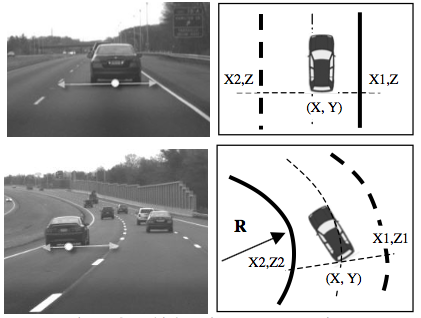
\includegraphics[scale=0.4]{figures/research_paper_figures/trajectory_multi-cue}
		\caption{Vehicle trajectory computation at straight and curved lanes \citep{multi-cue} }
		\label{fig:traj_multi-cue_image1}
	\end{minipage}\hfill
	\begin{minipage}{0.49\textwidth}
		\centering
		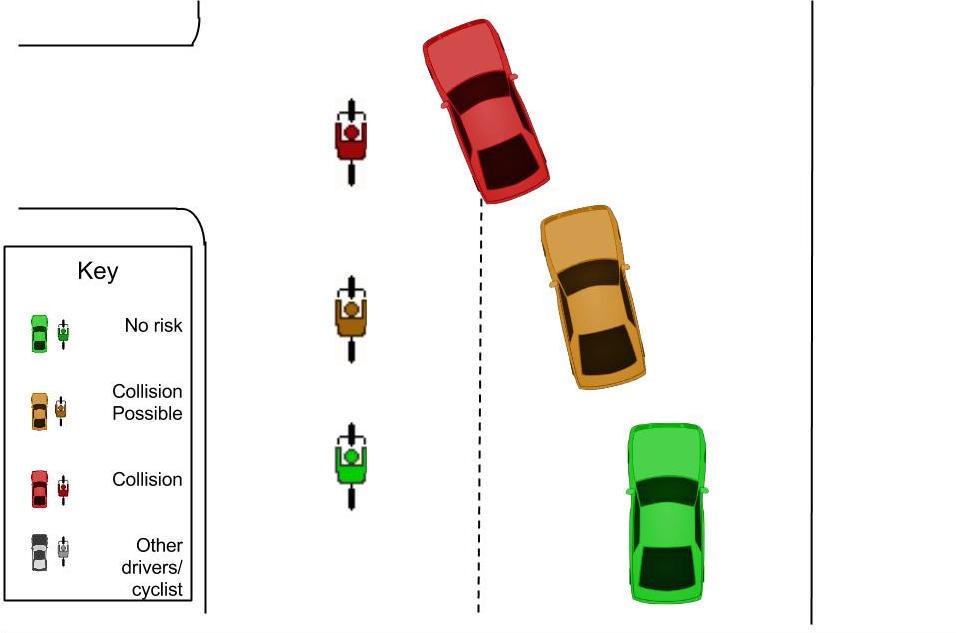
\includegraphics[scale=0.2]{figures/collision_avoidance_figures/Vehicle_changing_lane_into_the_path_of_a_cyclist}
		\caption{Cyclist and vehicle lane changing collision}
		\label{fig:change_lane_image}
	\end{minipage}
\end{figure}

Fig. ~\ref{fig:traj_multi-cue_image1} on page~\pageref{fig:traj_multi-cue_image1} shows the lane change tracking and prediction that this papers algorithms accomplish and Fig. ~\ref{fig:change_lane_image} on page~\pageref{fig:change_lane_image} shows, one of other, cyclist collisions that we want to prevent. This paper displays a high chance of solving this issue.



\subsubsection{Learning Multi-Lane Trajectories using Vehicle-Based Vision \citep{multi-lane_traj}}

Conclusion - decision complying with criteria at the start


%JACK brakes and why we decided to reject the automatic steering.


\chapter{Prototype Analysis}
\label{ch: prototype}
Prototyping is a very important part of the user-centred design process as this was the main opportunity for us to integrate user feedback into our design. This section will explain all of the major issues that we had to address because of our prototypes and the decisions we made as a result. There were two major components to our solution:
\begin{itemize}
  \item The bike hardware. Here we were trying to position all of the components (cameras, lights, battery, etc.) in the ideal position. We had to make sure that all of the components were positioned somewhere sensible and functional.
  \item The interface. These are the screens that the user directly interacts with to modify their settings and view statistics. The interface should allow the user to perform all of the key tasks with easy and efficiency.
\end{itemize}
We created some lo-fi prototypes for the interface using, the wireframing software, Balsamiq\cite{balsamiq}. This was particularly useful because it allowed us to create prototypes quickly and test them fairly easily. All of which helped us to receive, and then act on, user feedback. However it was not so easy for us to prototype the hardware due to our limited resources. We had to prototype the hardware using only sketches which was not ideal because it did not allow users to really get a feel for the design and how things interact. This meant we had to use our own knowledge of the product (and problem space) much more in this area.

\section{Prototype 1}
\label{sec:phones}
Analysis of the initial prototype sparked a discussion about the best medium for the interface. Initially we had decided to present the interface as a smartphone application, there were many reasons for this decision:
\begin{itemize}
  \item \textbf{Portability} The primary advantage of using a smartphone, from our point of view, was that it would allow users to change their settings on-the-go. We felt that this would be hugely beneficial for users if they can change their settings while they are away from the bike and have them automatically download whenever they start to ride. 
  \item \textbf{Cost} Having users simply download a free application for their existing technology significantly lowers the production cost of the bike. The software would need to be developed in any event, however it would save on hardware costs. 
  \item \textbf{Familiarity} Products tend to be much easier to use if they use elements that the user is familiar with and most smartphone users are very familiar with downloading and using applications for their phone.
  \item \textbf{Battery} One of the major problems that we identified early on was the battery life of the bike. By using a separate device, such as a smartphone, the interface will not drain the bike's inbuilt battery.
\end{itemize}
Following the initial prototype we considered switching this to an inbuilt, custom-made device. We felt that this would simplify the product overall as it would not rely on any external technologies to work and would be single platform and single form-factor. Also, it could alleviate some of the security concerns that come with pairing phones to the bike - this is a tough problem due to the fact it required multiple users being able to pair with multiple bikes securely. An added benefit of this would be connection speed - a phone would need to use a bluetooth connection whereas an inbuilt device could quite easily be hardwired into CPU.

After taking all of this into account we eventually decided to stick with using a smartphone interface. The reasons for this being:
\begin{itemize}
  \item \textbf{Security} Although an built device may make application security easier to achieve, a smartphone based interface would improve the physical security of the bike. As the smartphone would obviously be removable this removes valuable looking items from show making the bike less likely to be stolen.
  \item \textbf{Integration} We felt that it is important that this design is future-proof and easy to build upon. Many current bicycle applications integrate with other applications such as Facebook, Twitter and Google+. Applications for all of these already exist on all of the major smartphone operating systems which would make it simple to integrate with them in the future.
  \item \textbf{Internet access} The \textit{key} reason for choosing a smartphone based interface was that some of the intended features would be very difficult, or maybe impossible, without it. The user login feature, for example, will require internet access - this can be achieved easily with smartphone tethering. However, without a smartphone would require some sort of mobile internet subscription or other way to connect to the 3G network.
\end{itemize}
This discussion also helped point out some of other design problems that we would need to address in the next prototype; the biggest of these being the phone battery. If a user were to cycle somewhere and then before cycling back their smartphone ran out of battery they would not be able to unlock the bike to cycle home. This could have a been major design flaw if left unaddressed. Another potential problem that was overlooked in the initial design is that phones do not conform to one particular shape or size; the latest iPhone 6 plus is 6.22 x 3.06 inches while the Sony Xperia M measures 4.88 x 2.44 inches.

There was also some issues pointed out by users. Many asking ``how does it save my settings?" or ``how do you log in?". This was something that was forgotten in the initial design and would need to be addressed in the next iteration. Also, some users found that the bike battery level was not prominent enough on the interface. 
\section{Prototype 2}

\chapter{Final Design}
\section{Overview of User Interface}
\section{Screen Images}
\section{Screen Objects and Actions}

\chapter{Conclusion}

\part*{Appendices}
\appendix
%TOM: need to write why we decided on electronic brakes...
\chapter{Electronic Braking System}
\section{Current Technology}

\begin{figure}[h]
\centering
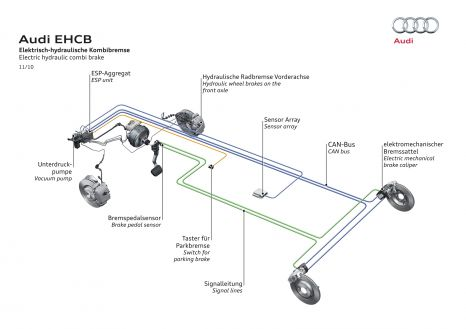
\includegraphics[scale=0.7]{figures/electronic_braking/audi_EHCB_1}
\caption{  \citep{audi_ehcb_1}}

\end{figure}

\begin{figure}[h]
\centering
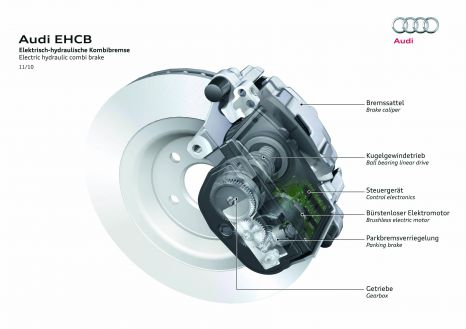
\includegraphics[scale=0.7]{figures/electronic_braking/audi_EHCB_2}
\caption{Audi Electric Hydraulic combo Brakes  \citep{audi_ehcb_2}}
\end{figure}



\chapter{Research Report}
In this mini-report we will be showing the preliminary research that we did before designing our final solution. The overall aim of doing this research was to discover the best way in which to improve safety in cycling. In order to do this we analysed a range of statistics as well as speaking directly to different stakeholders and ...
\newpage
\section{Statistics}
\subsection{Number of cyclists}
According to the most recent National Travel Survey statistics (2013) \textbf{43\% of the population owns a bicycle} 
\subsection{Accidents}
\subsection{Fatalities}
\subsection{Road types}
\subsection{Time of day}
\subsection{Vehicles}
\newpage
\section{Questionnaires}
\newpage
\section{Current products}
We looked at a whole variety of safety products currently on the market for cars and trucks as well as bikes. The reason for this was to see why certain products were succeeding and which features of these products we might wish to incorporate into our solution. We also looked at failed products to get an idea of the potential design problems we might encounter later on as well as allowing us to rule out some of the previously attempted solutions.
\subsection{Bike Lights}
The most basic, and often the only, form of bike safety used is the bike light; this is used to make a cyclist visible to all road users allowing them to take the appropriate action. In the UK front and rear bike lights (and reflectors) are required by law between sunset and sunrise. This is governed by the Road Vehicle Lighting Regulations 1989\cite{rvlr} and if our solution were to use in-built lighting we would have to make sure that we complied with these regulations. This poses an interesting problem because different sets of regulations exist in different countries; most manufacturers actually tend to ignore the UK's regulations because of the relatively small cycling population and also the regulations are considered by many to be old and outdated. In practice as long as a cyclist has lights of some description on both the front and rear of their bike they are unlikely to be questioned by police. 

Bike lights come in many different forms but, according to retailer that we spoke to, LED currently dominates the market. They are small, cheap, last forever and they provide a lot of light! The retailer also told us that it is important for lights to have a wide field as well as to be bright. This allows cyclists to be seen even by people not directly in front or behind; for example cars waiting to pull out of a junction.

\paragraph{Revolight} A slightly different take on the bike light is the Revolight\cite{revolight}; here the light is incorporated the bike's tyres. The lights are mounted all around the wheel and are timed to only illuminate when facing the front or rear of the bicycle using a fork-mounted magnet and integrated accelerometer. The primary benefit of this is that it gives total 360\degree vision of the bike.

This started as a Kickstarter project\cite{revo_ks} in 2011 and has since reached it's goal and is now on sale for \$199. There is no sales information readily available nor any statistics about how operationally successful this product has been. However the Revolight design has won several awards from cycling publications\cite{revo_awards} and has recently received \$1 million in funding from investors so it appears that this product has been very successful.

\paragraph{Blaze Laserlight}
The Blaze Laserlight\cite{laserlight} projects a green laser image of a bicycle up to 6m ahead of the cyclist. The idea of this product is to cut down on accidents where the cyclist is caught in a vehicles blind spot at the time of them making a manoeuvre into their path. According to the creators of the Blaze Laserlight - 79\% of accidents happen this way. 

One particular design decision that was made by the people at Blaze was to have the light project in green, the reason for this is because humans are most sensitive to light between 490-560 nm (green light). This could be something to think about if we incorporate lights into our design.

This product tries to avoid accidents by making other road users more aware of cyclist. However it has a few problems:
\begin{itemize}
\item It will not be as effective at night. This technology is based on LED bike lights which are only effective in low light.
\item It still puts the responsibility on other road users. It will not protect the cyclist from unobservant road users and it most likely these people who are causing these accidents in the first place.
\end{itemize}

\paragraph{XFire}
The XFire\cite{xfire} product works similarly to the Blaze Laserlight by projecting light onto the road. However instead of projecting an image of the bike it projects a bike lane. The idea here is to buy cyclists more space during overtaking manoeuvres, particularly on roads where there is no cycle lane. This has the added advantage that all road users are familiar with bike lanes and how they operate. 

This product is relatively cheap, retailing online at \$29.99 however has the same disadvantages as the Blaze Laserlight

\subsection{Helmets}
Probably the next most common safety product used at the moment is the helmet. The helmet is a impact reduction approach to managing the risk; it will not help to prevent an accident from occurring but it may stop an accident from being fatal. Currently helmets are not required by UK law however according to government guidelines, ``You \textit{should} wear a cycle helmet which conforms to current regulations, is the correct size and securely fastened"\cite{helmet_gov}.

\paragraph{Hovding airbag}According to, former professional cyclist, Michael Hutchinson ``The most outstanding design flaw with the traditional polystyrene helmet is that it messes up people's hair, it's sweaty on the head, also a lot of people don't like the look of bike helmets."\cite{hutch} The ``Hovding airbag" \cite{hovding} is an invisible helmet that attempts to overcome these issues. It is an airbag fitted into a neck collar and uses sensors and an algorithm to detect a fall. Once detected, it inflates over the user’s head like a hood, protecting the users head from impact damage.

This has been the only noticeable innovation in bike helmets and for this reason it is unlikely that helmets will form and significant part of our solution. However, this particular product does show the importance of style as well as safety and that it something we will need to keep in mind throughout the design process.

\subsection{Mobile apps}
Mobile apps are now used throughout everyday life due to their accessibility and ability to interact with the outside world. This ability to interact might be something that we can utilise in our product. Here we looked at some of the ways in which mobile apps are currently being used by cyclists.

\paragraph{Bike Doctor} One example of such an app is the `Bike Doctor'\cite{bike_doctor} which is supposed to be a personal bike mechanic. It contains many bike maintenance guides and is designed to provide easy to follow instructions on how to repair and maintain particular parts of the bicycle yourself. It was designed to be ideal for beginners but also as a handy reference guide for more experienced cyclists. This concept may be something to consider as it is a trusted app by over 14,000 cyclists and having a well maintained bike would prevent a chance of a breakdown during cycling and causing an injury during cycling. 

Something that this app does not do is detects faults in the bike to give tailored advice, similarly to the dashboard lights in cars. This would be a very useful feature that would improve bike safety. A problem with this app is that it will not prevent accidents that are not the fault of the cyclist; which our earlier research showed are the majority.

\paragraph{Strava} A particularly successful app that is used by cyclists is Strava\cite{strava}. Strava is predominantly a tracking application/social network where users can share their routes with other cyclists. A feature of Strava that we found particularly interesting was the in built challenges, where users earn recognition amongst their peers for cycling a particular distance or route. This really encourages people to cycle and moreover to keep up their cycling habit. Strava also has potential safety benefits because users can use recommended routes which should be safer to ride, however this is not the primary focus of Strava.

It does seem that the primary audience of this app is people who cycle for recreation or fitness, whereas we are predominantly targeting people who cycle for commuting or transport. However, it may be possible to overcome this problem by analysing routes of all cyclists to find the best possible routes to a given location.

%FlyKly Wheel

\newpage
\section{Car technologies}
Looking at, and mimicking, successful innovations in car safety technology was one of the predominant methods for com
\newpage
\section{Other research}
\subsection{Route planning}
If we are to incorporate some sort of safety based route planning into our final solution we will need some method for determining the relative safety of any given road/route.

\subsubsection{User Perception}
One way to do this is to try and to model a cyclist's perception. An attempt at this is the Bicycle Compatibility Index (BCI) [1]; an American idea from 1998 as part of an initiative to double number of trips made by cycling or walking and to simultaneously reduce accidents by 10\%. The BCI is intended to be a measure of how well suited any particular road is to accommodate both motorists and cyclists.

The BCI was developed using the perspectives of cyclists; asking them to view videoclips and evaluate how comfortable they would be cycling on that road in the conditions shown. The index is then calculated using the method show in in figure \ref{fig:bci_calc}.
\begin{figure}
\centering
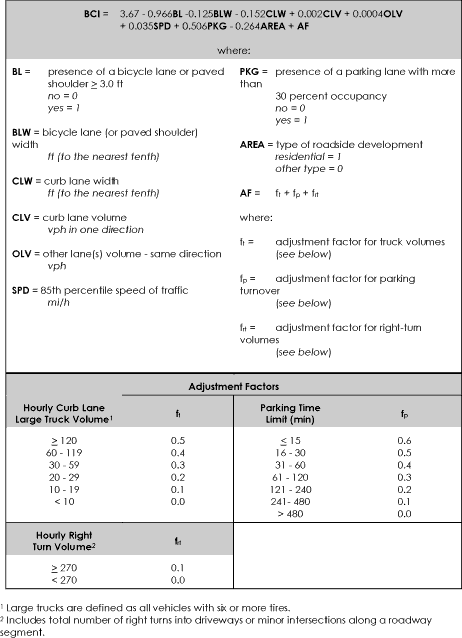
\includegraphics[scale=0.5]{figures/research_report/bci}
\caption{The calculation for the Bicycle Compatibility Index}
\label{fig:bci_calc}
\end{figure}

Fairly obviously, the presence of a dedicated cycle lane wider than 0.9m is the most significant factor on the comfort of cyclists, along with the width of the inside lane and cycle lanes. Interestingly though, according to the research, the speed of traffic is considered more important (0.022) than the volume of traffic (0.002); this would indicate that it would be better for cyclists to travel on gridlocked busy roads during rush hour rather than the back streets which although quieter are more likely to have traffic flowing faster.

The BCI also gives an indication towards what an index value means regarding how compatible the road is, this is shown in figure \ref{fig:bci_los}:

\begin{figure}
\centering
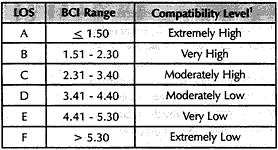
\includegraphics[scale=0.7]{figures/research_report/bci_los}
\caption{The}
\label{fig:bci_los}
\end{figure}

\chapter{Stakeholder Map}
\label{ch:stakeholders}
On the following pages is a stakeholder map and analysis showing all of the people who may be affected by this project. 

Some of the stakeholders shown are directly affected, cyclists for example. Whereas others are only affected as a secondary effect.

Some may be positively affected by the project and other negatively. In the analysis we will show the likely reactions of some of the key holders and the reasons for this reaction.
\newpage
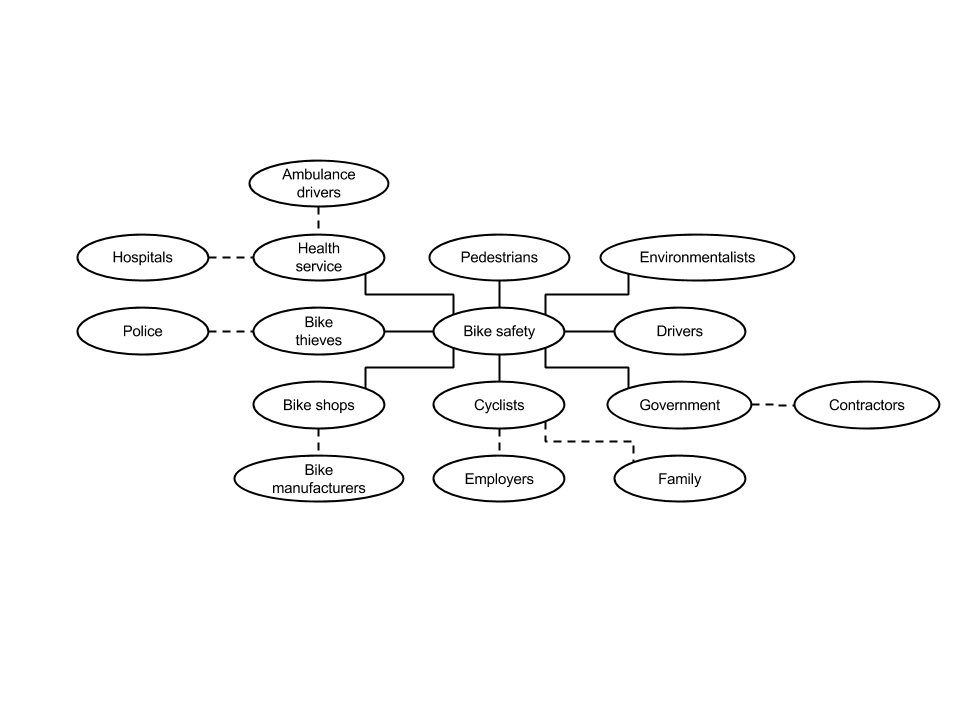
\includegraphics[scale=0.5, angle=90]{figures/stakeholder_map}

\chapter{Prototype 1}
\begin{figure}
\centering
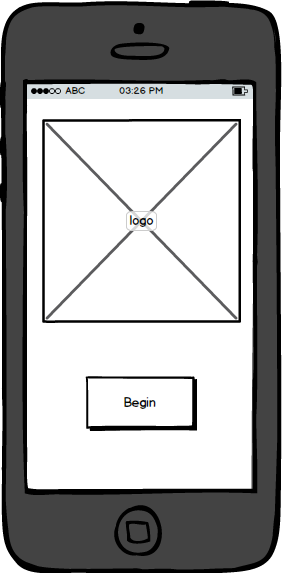
\includegraphics[scale=0.]{figures/prototype_1/title}
\caption{Title screen}
\end{figure}
\clearpage
\begin{figure}
\centering
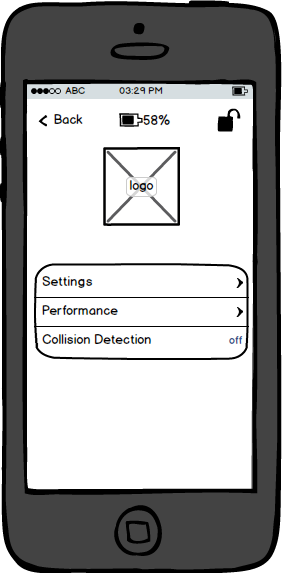
\includegraphics[scale=0.9]{figures/prototype_1/main_menu}
\caption{Main menu}
\end{figure}
\clearpage
\begin{figure}
\centering
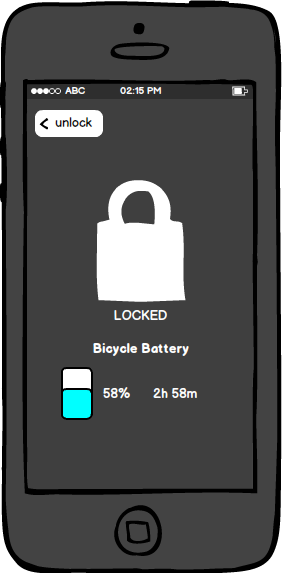
\includegraphics[scale=0.9]{figures/prototype_1/locked}
\caption{Screen that displays when bike is locked}
\end{figure}
\clearpage
\begin{figure}
\centering
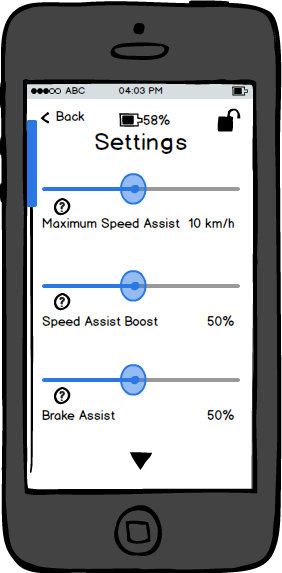
\includegraphics[scale=0.9]{figures/prototype_1/settings}
\caption{Screen allowing the user to adjust settings}
\end{figure}
\clearpage
\begin{figure}
\centering
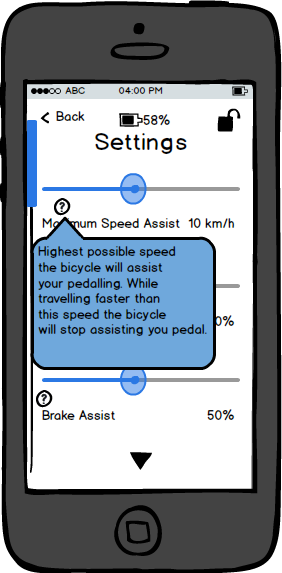
\includegraphics[scale=0.9]{figures/prototype_1/settings_help_1}
\caption{Alert box explain what the setting does}
\end{figure}
\clearpage
\begin{figure}
\centering
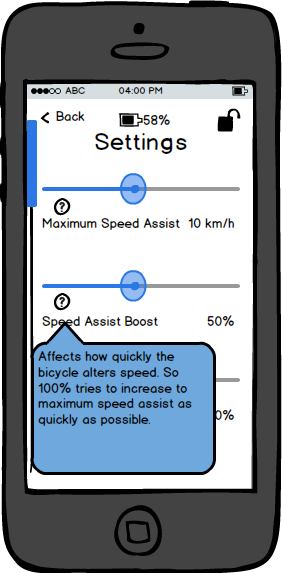
\includegraphics[scale=0.9]{figures/prototype_1/settings_help_2}
\caption{Alert box explain what the setting does}
\end{figure}
\clearpage
\begin{figure}
\centering
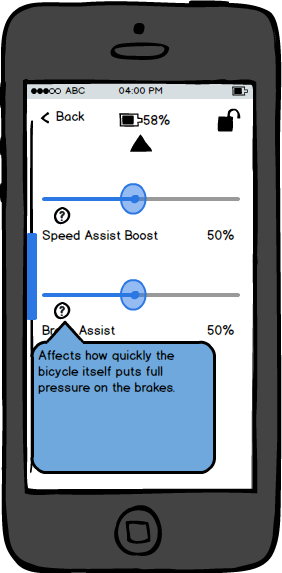
\includegraphics[scale=0.9]{figures/prototype_1/settings_help_3}
\caption{Alert box explain what the setting does}
\end{figure}
\clearpage
\begin{figure}
\centering
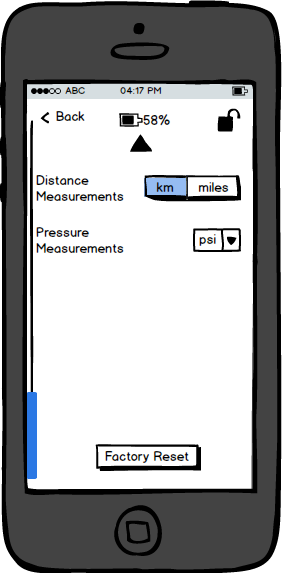
\includegraphics[scale=0.9]{figures/prototype_1/settings_2}
\caption{Some more settings}
\end{figure}
\clearpage
\begin{figure}
\centering
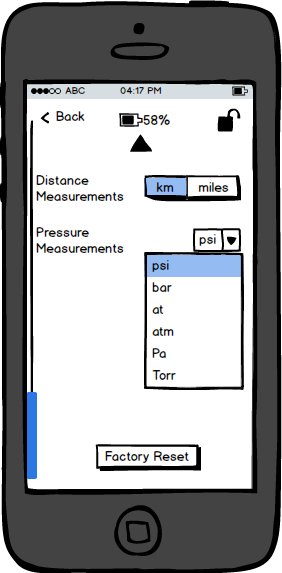
\includegraphics[scale=0.9]{figures/prototype_1/settings_2_check}
\caption{Dropdown menu}
\end{figure}
\clearpage
\begin{figure}
\centering
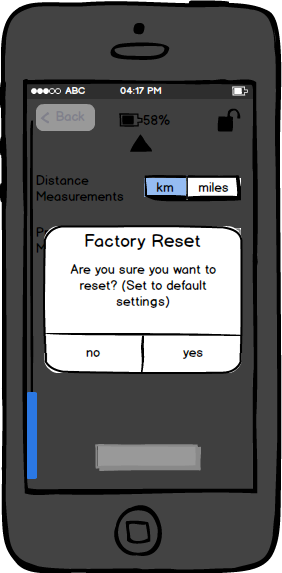
\includegraphics[scale=0.9]{figures/prototype_1/factory_settings}
\caption{Warning when performing a factory reset}
\end{figure}
\clearpage
\begin{figure}
\centering
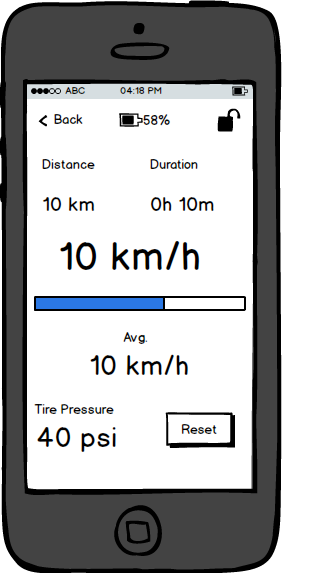
\includegraphics[scale=0.9]{figures/prototype_1/perf}
\caption{The performance screen. This is the main riding screen}
\end{figure}
\clearpage
\begin{figure}
\centering
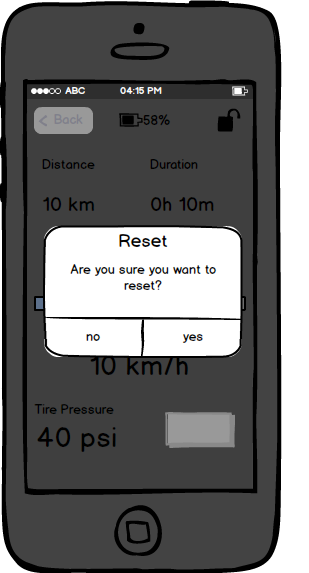
\includegraphics[scale=0.9]{figures/prototype_1/reset_perf}
\caption{Warning when resetting performance stats}
\end{figure}
\clearpage
\begin{figure}
\centering
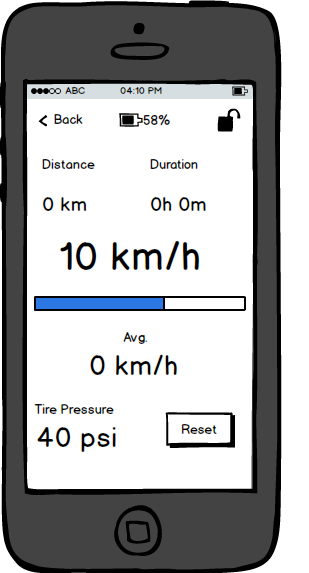
\includegraphics[scale=0.9]{figures/prototype_1/resetted}
\caption{The performance screen following a reset}
\end{figure}
\clearpage
\begin{figure}
\centering
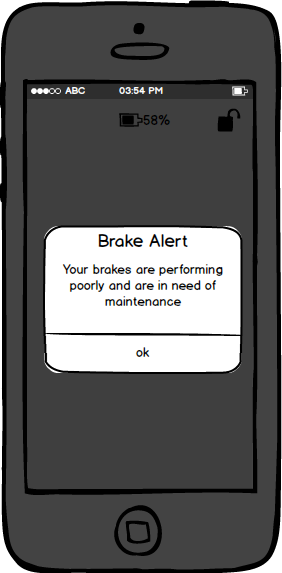
\includegraphics[scale=0.9]{figures/prototype_1/brake_maint}
\caption{A brake maintenance alert, this could display over any screen}
\end{figure}
\clearpage
\begin{figure}
\centering
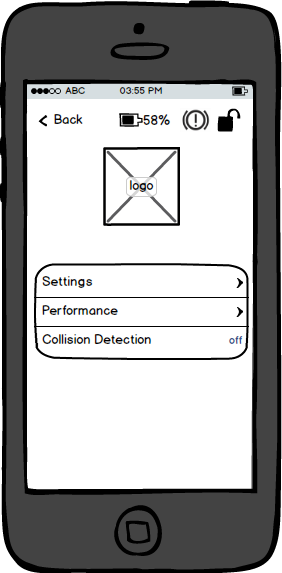
\includegraphics[scale=0.9]{figures/prototype_1/main_menu_warn}
\caption{The main menu showing the warning icon at the top}
\end{figure}
\clearpage
\begin{figure}
\centering
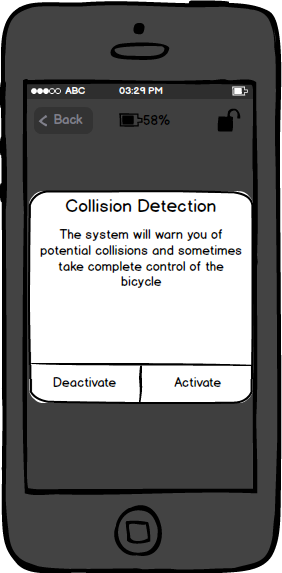
\includegraphics[scale=0.8]{figures/prototype_1/collision_activate}
\caption{Warning explaining collision detection system before it is de/activated}
\end{figure}
\clearpage
\begin{figure}
\centering
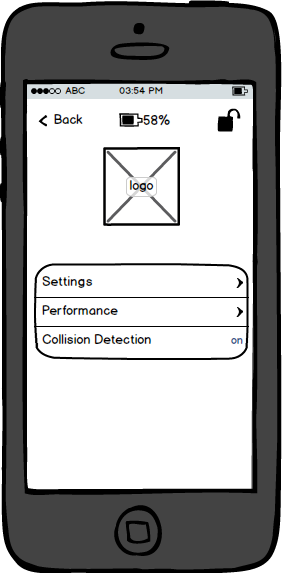
\includegraphics[scale=0.9]{figures/prototype_1/collision_on}
\caption{Main menu screen showing that collision detection is on}
\end{figure}
\clearpage
\begin{figure}
\centering
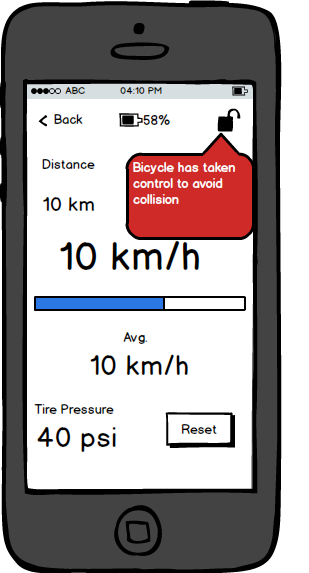
\includegraphics[scale=0.8]{figures/prototype_1/control_alert_perf}
\caption{Alert showing that the collision detection system has started to take control. Could display on any screen}
\end{figure}
\clearpage
\begin{figure}
\centering
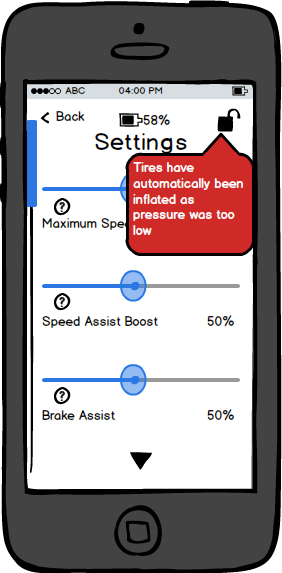
\includegraphics[scale=0.9]{figures/prototype_1/inflation_settings}
\caption{Alert showing that automatic tire-inflation has been activated. Could display on any screen}
\end{figure}
\clearpage
\begin{figure}
\centering
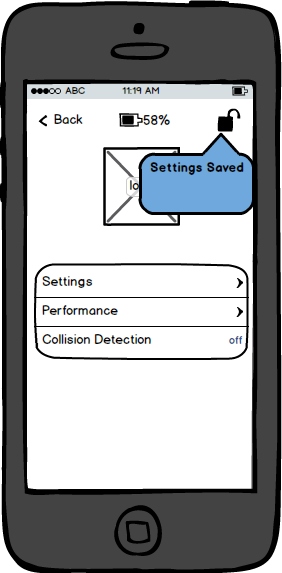
\includegraphics[scale=0.9]{figures/prototype_1/settings_saved}
\caption{Alert showing that the updated settings have been saved}
\end{figure}
\clearpage

\chapter{Prototype 2}
%\input{chapters/appendix}

\bibliographystyle{plainnat}
\bibliography{bibliography}
\end{document}
